\chapter{PNb data analysis}
\label{chapter:analysis_pNb}
Complemantary to the pp exerimewnt a data from pNb experiment was analized. Mian scope of the studies was the same, aldough differences in physiscal sytuation has forced some minnor changes in used methods. As a result inclusive \css for $\Ls$ together with the reference state $\Lz \Kz$ were measured and compared to the previous HADES studies \cite{hades_Sz_pNb,hades_Lp_femtoscopy_pNb,hades_arnold_pNb,hades_Ksi_pNb}. It allows to extend knowladge about hyperons into a pNb reactions and to point key diffrences between proton-proton and pronon-nucleon reactions.
\section{Data from pNb experiment}
The p (3.5 GeV) +Nb  experiemnt took place in ???.


\section{Identyfication and data selection}
The used identyfication and selection algorithms were the same as in case of a pp data analaysis. However in proton-nucleus reaction it is impossible to directly use the energy-momentum conservation rule. They are two main obstacles: part of four-momentum may be transfered to the nucleus as a recoil and nuceons in nucleus are not in rest. All together prevents from a use of the missing mass cut. As a replacement a set of hard cuts was applayed.

\section{The $\Lz$ Reconstruction}
The main tool for $\Lz$ reconstruction stays the same as for in chapter \ref{chapter:analysis}. It is a neural network trained in a data-driven maner. Aldouth for a good signal extraction a set of additional pre-cuts was necessary. They are summerized in tab. ???

After applaying all cuts described in above table a signal~to~background ratio ??? was obtained. The result is shown in fig. \ref{fig:L1116SB_pNb}.
\begin{figure}[ht]
  \centering
  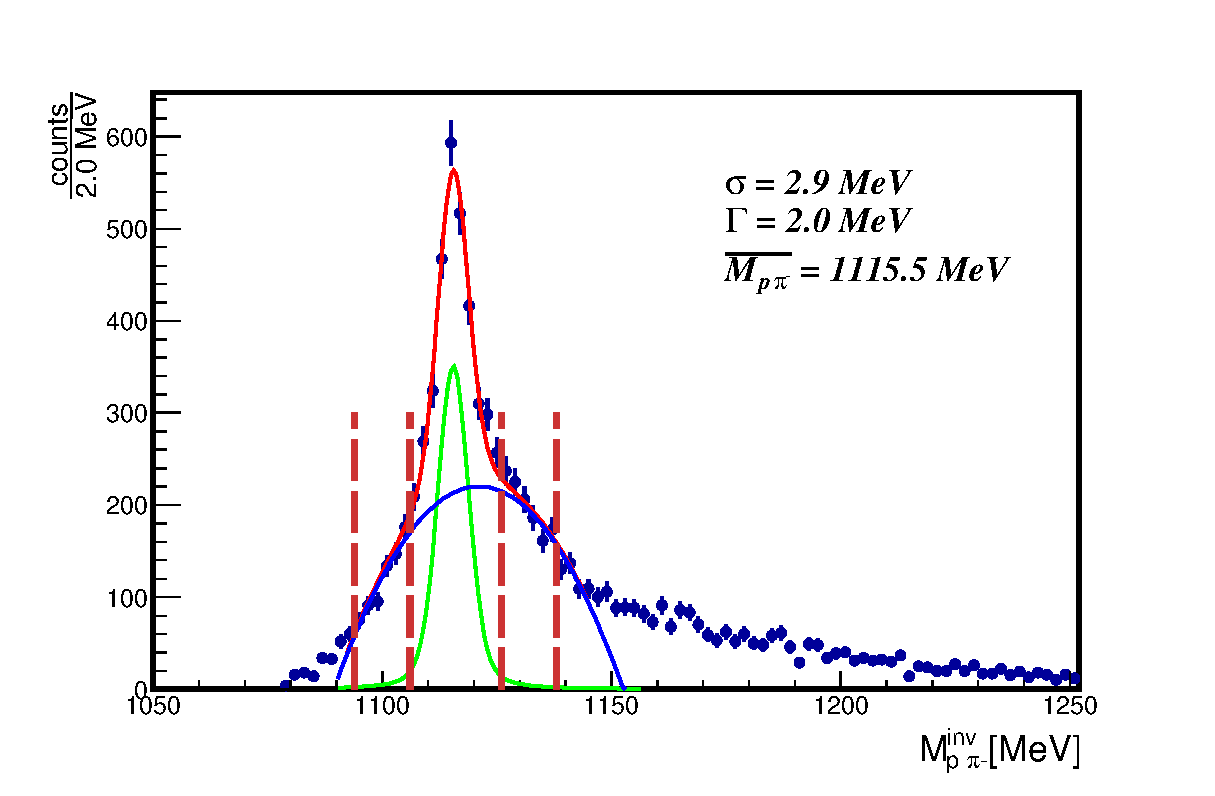
\includegraphics[width=0.7 \linewidth]{Chapter_analysisPNb/Lz.eps}
  \caption{The $\Lz$ spectrum after a neural network analysis obtained for pNb experiment. Color coding the same as in fig. \ref{fig:L1116SB}, vertical lines denotes regions of a side-band and were adjusted for pNb exclusively.}
  \label{fig:L1116SB_pNb}
\end{figure}

\section{The $\Lz \Kz $reconstruction}
\begin{figure}[ht]
  \centering
  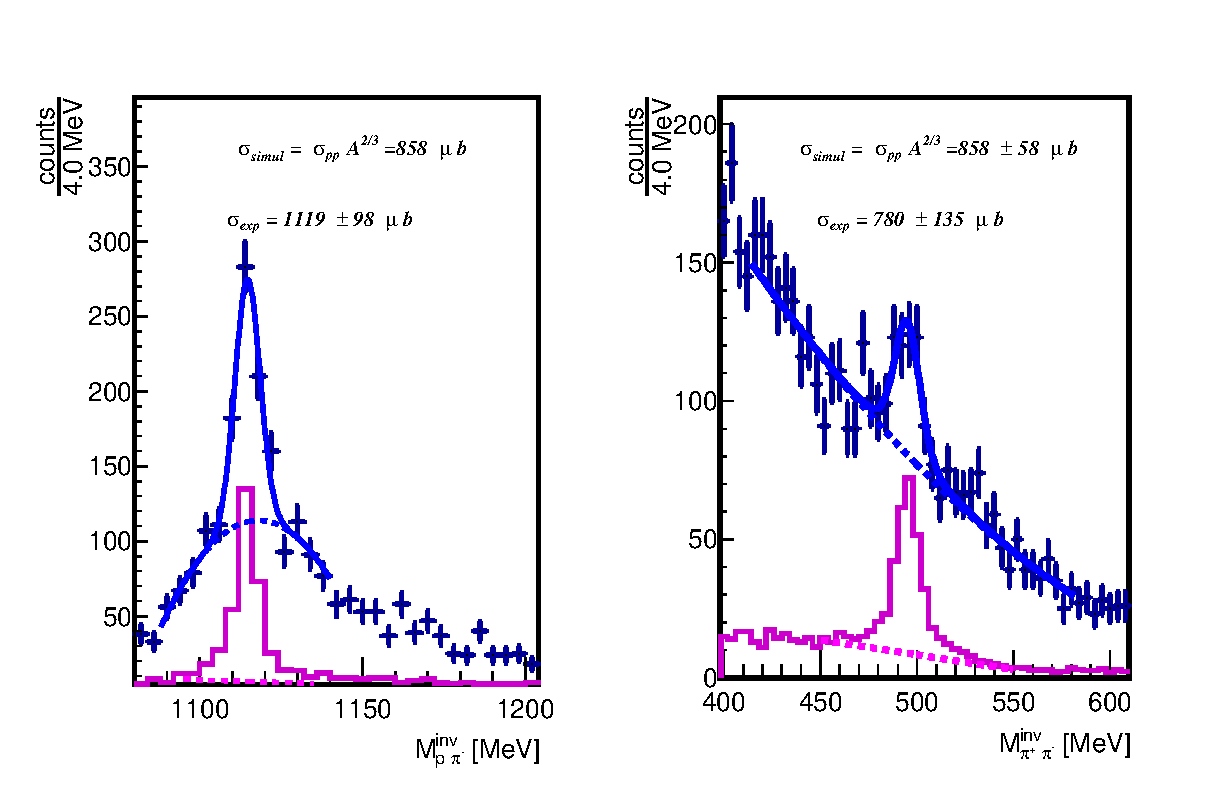
\includegraphics[width=0.9 \linewidth]{Chapter_analysisPNb/LK0.eps}
  \caption{The inclusive $\Lz \Kz$ spectrum obtained for pNb experiment. The \css for the simulation was scaled up by a factor $A^{2/3}$ compare values measured in pp reactions}
  \label{fig:LK0_pNb}
\end{figure}

\section{The $\Ls$ Reconstruction}



\subsection{Event mixing}


\subsection{Cross-section and extraction differential analysis}
\begin{figure}[ht]
  \centering
  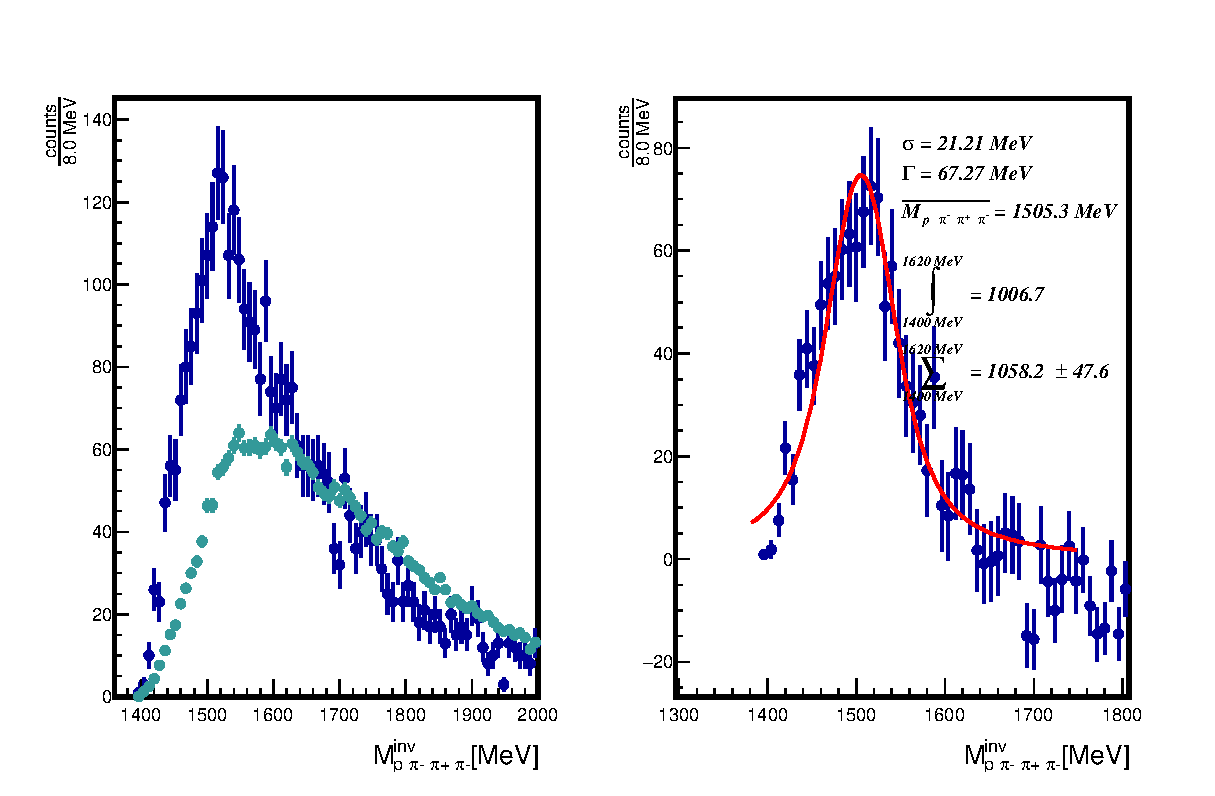
\includegraphics[width=0.9 \linewidth]{Chapter_analysisPNb/L1520.eps}
  \caption{a}
  \label{fig:L1520_pNb}
\end{figure}

\begin{figure}[ht]
  \centering
  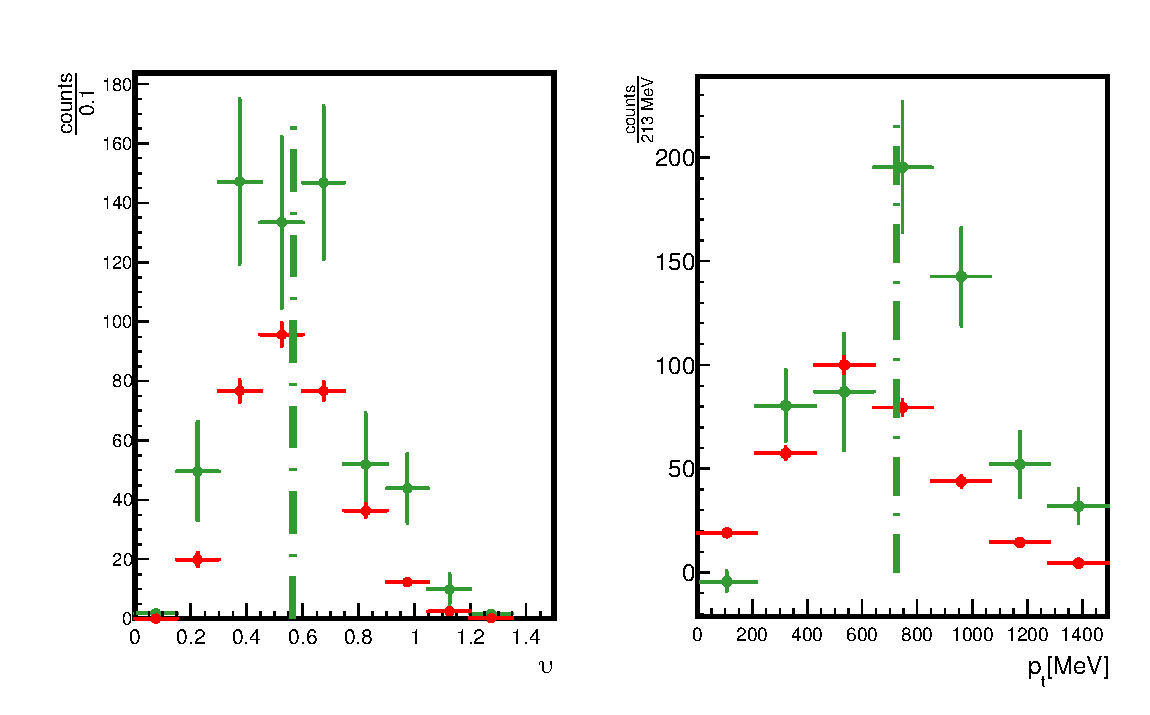
\includegraphics[width=0.9 \linewidth]{Chapter_analysisPNb/YPt.eps}
  \caption{b}
  \label{fig:YPt_pNb}
\end{figure}

\subsection{Analysis of a $\pip \pim$ spectrum}

\section{Comparison with results from pp data}